\documentclass[11pt]{article}
% https://www.gradescope.com/help#help-center-item-answer-formatting-guide
\usepackage{microtype}
\usepackage{graphicx}
\usepackage{wrapfig}
\usepackage{url}
\usepackage{wrapfig}
\usepackage{color}
\usepackage{marvosym}
\usepackage{enumerate}
\usepackage{subfigure}
\usepackage{tikz}
\usepackage[fleqn]{amsmath}
\DeclareMathOperator*{\argmax}{argmax}
\DeclareMathOperator*{\argmin}{argmin}
\usepackage{amssymb}
\usepackage{hyperref}
\usepackage[many]{tcolorbox}
\usepackage{lipsum}
\usepackage{float}
\usepackage{trimclip}
\usepackage{listings}
\usepackage{environ}% http://ctan.org/pkg/environ
\usepackage{wasysym}
\usepackage{array}
\usepackage{bbm}
\usepackage{enumitem}

\oddsidemargin 0mm
\evensidemargin 5mm
\topmargin -20mm
\textheight 240mm
\textwidth 160mm

\newcommand{\vwi}{{\bf w}_i}
\newcommand{\vw}{{\bf w}}
\newcommand{\vx}{{\bf x}}
\newcommand{\vy}{{\bf y}}
\newcommand{\vxi}{{\bf x}_i}
\newcommand{\yi}{y_i}
\newcommand{\vxj}{{\bf x}_j}
\newcommand{\vxn}{{\bf x}_n}
\newcommand{\yj}{y_j}
\newcommand{\ai}{\alpha_i}
\newcommand{\aj}{\alpha_j}
\newcommand{\X}{{\bf X}}
\newcommand{\Y}{{\bf Y}}
\newcommand{\vz}{{\bf z}}
\newcommand{\msigma}{{\bf \Sigma}}
\newcommand{\vmu}{{\bf \mu}}
\newcommand{\vmuk}{{\bf \mu}_k}
\newcommand{\msigmak}{{\bf \Sigma}_k}
\newcommand{\vmuj}{{\bf \mu}_j}
\newcommand{\msigmaj}{{\bf \Sigma}_j}
\newcommand{\pij}{\pi_j}
\newcommand{\pik}{\pi_k}
\newcommand{\D}{\mathcal{D}}
\newcommand{\el}{\mathcal{L}}
\newcommand{\N}{\mathcal{N}}
\newcommand{\vxij}{{\bf x}_{ij}}
\newcommand{\vt}{{\bf t}}
\newcommand{\yh}{\hat{y}}
\newcommand{\code}[1]{{\footnotesize \tt #1}}
\newcommand{\alphai}{\alpha_i}
\newcommand{\defeq}{\overset{\text{def}}{=}}
\renewcommand{\vec}[1]{\mathbf{#1}}



\bgroup
\def\arraystretch{1.5}
\newcolumntype{x}[1]{>{\centering\arraybackslash\hspace{0pt}}p{#1}}
\newcolumntype{z}[1]{>{\centering\arraybackslash}m{#1}}

%Arguments are 1 - height, 2 - box title
\newtcolorbox{textanswerbox}[2]{%
 %width=\textwidth,
 colback=white,colframe=blue!30!black,floatplacement=H,height=#1,title=#2,clip lower=true,before upper={\parindent0em}}

 \newtcolorbox{eqanswerbox}[1]{%
 width=#1,colback=white,colframe=black,floatplacement=H,height=3em,sharp corners=all,clip lower=true,before upper={\parindent0em}}

 %Arguments are 1 - height, 2 - box title
 \NewEnviron{answertext}[2]{
        \noindent
        \marginbox*{0pt 10pt}{
        \clipbox{0pt 0pt 0pt 0pt}{
        \begin{textanswerbox}{#1}{#2}
        \BODY
        \end{textanswerbox}
        }
        }
}

%Arguments are 1 - height, 2 - box title, 3 - column definition
 \NewEnviron{answertable}[3]{
        \noindent
        \marginbox*{0pt 10pt}{
        \clipbox{0pt 0pt 0pt 0pt}{
        \begin{textanswerbox}{#1}{#2}
                \vspace{-0.5cm}
                        \begin{table}[H]
                        \centering
                        \begin{tabular}{#3}
                                \BODY
                        \end{tabular}
                        \end{table}
        \end{textanswerbox}
        }
        }
}

 %Arguments are 1 - height, 2 - box title, 3 - title, 4- equation label, 5 - equation box width
 \NewEnviron{answerequation}[5]{
        \noindent
        \marginbox*{0pt 10pt}{
        \clipbox{0pt 0pt 0pt 0pt}{
        \begin{textanswerbox}{#1}{#2}
                \vspace{-0.5cm}
                        \begin{table}[H]
                        \centering
                \renewcommand{\arraystretch}{0.5}% Tighter

                        \begin{tabular}{#3}
                                #4 =    &
                        \clipbox{0pt 0pt 0pt 0pt}{

                        \begin{eqanswerbox}{#5}
                                $\BODY$
                        \end{eqanswerbox}
                        } \\
                        \end{tabular}
                        \end{table}

        \end{textanswerbox}
        }
        }
}

 %Arguments are 1 - height, 2 - box title
 \NewEnviron{answerderivation}[2]{
        \noindent
        \marginbox*{0pt 10pt}{
        \clipbox{0pt 0pt 0pt 0pt}{
        \begin{textanswerbox}{#1}{#2}
        \BODY
        \end{textanswerbox}
        }
        }
}

\newcommand{\Checked}{{\LARGE \XBox}}%
\newcommand{\Unchecked}{{\LARGE \Square}}%
\newcommand{\TextRequired}{{\textbf{Place Answer Here}}}%
\newcommand{\EquationRequired}{\textbf{Type Equation Here}}%


\newcommand{\answertextheight}{5cm}
\newcommand{\answertableheight}{4cm}
\newcommand{\answerequationheight}{2.5cm}
\newcommand{\answerderivationheight}{14cm}

\newcounter{QuestionCounter}
\newcounter{SubQuestionCounter}[QuestionCounter]
\setcounter{SubQuestionCounter}{1}

\newcommand{\subquestiontitle}{Question \theQuestionCounter.\theSubQuestionCounter~}
\newcommand{\newquestion}{\stepcounter{QuestionCounter}\setcounter{SubQuestionCounter}{1}\newpage}
\newcommand{\newsubquestion}{\stepcounter{SubQuestionCounter}}


\lstset{language=[LaTeX]TeX,basicstyle=\ttfamily\bf}

\pagestyle{myheadings}
\markboth{Homework 4}{Spring 2020 CS 475/675 Machine Learning: Homework 4}

\title{CS 475 Machine Learning: Homework 4\\
Clustering, EM, Dimensionality Reduction,\\Graphical Models\\
Analytical Problems \\
\Large{Due: Wednesday April 15, 2020, 11:59 pm}\\
50 Points Total \hspace{1cm} Version 1.0}
\author{YOUR\_NAME (YOUR\_JHED)}
\date{}

\begin{document}
\maketitle
\thispagestyle{headings}

\section*{Instructions }
We have provided this \LaTeX{} document for turning in this homework. We give you one or more boxes to answer each question.  The question to answer for each box will be noted in the title of the box.

 $\newline${\bf Other than your name, do not type anything outside the boxes. Leave the rest of the document unchanged.}

$\newline$\textbf{Do not change any formatting in this document, or we may be unable to
  grade your work. This includes, but is not limited to, the height of
  textboxes, font sizes, and the spacing of text and tables.  Additionally, do
  not add text outside of the answer boxes. Entering your answers are the only
  changes allowed.}


$\newline$\textbf{We strongly recommend you review your answers in the generated PDF to
  ensure they appear correct. We will grade what appears in the answer boxes in
  the submitted PDF, NOT the original latex file.}

\pagebreak

% \newquestion
\section*{ Notation}
{
\begin{table}[h]
% \caption{Notation.}\smallskip
\centering
\resizebox{.95\columnwidth}{!}{
\smallskip\begin{tabular}{r l}
\(\vec{x_i}\) & One input data vector. \(\vec{x_i}\) is \(M\) dimensional.
                                    \(\vec{x_i} \in \mathbb{R}^{1 \times M}\).  \\ &
                                    We assume $\vec{x_i}$ is augmented with a  $1$ to include a bias term. \\ \\
\(\vec{X}\) &   A matrix of concatenated \(\vec{x_i}\)'s. There are \(N\) input vectors, so \(\vec{X} \in \mathbb{R}^{N \times M}\) \\ \\
\(y_i\) & The true label for input vector \(\vec{x_i}\). In regression problems, \(y_i\) is a continuous value. \\ & In general \(y_i\) can be a vector, but for now we assume \(y_i\) is a scalar. \(y_i \in \mathbb{R}^1\). \\ \\

\(\vec{y}\) &   A vector of concatenated \(y_i\)'s. There are \(N\) input vectors, so \(\vec{y} \in \mathbb{R}^{N \times 1}\) \\ \\

\(\vec{w}\) & A weight vector. We are trying to learn the elements of \(\vec{w}\). \\ & \(\vec{w}\) is the same number of elements as \(\vec{x_i}\) because we will end up computing the dot product \(\vec{x_i} \cdot \vec{w}\). \\ & \(\vec{w} \in \mathbb{R}^{M \times 1}\). We assume the bias term is included in \(\vec{w}\). \\ \\
 
% \(E_D(\vec{w})\) & The loss due to the model fit. \\ \\
% \(E_\vec{w}(\vec{w})\) & The regularization term.  \\ \\

 Notes: & In general, a lowercase letter (not boldface), $a$, indicates a scalar. \\
  & A boldface lowercase letter, $\vec{a}$, indicates a vector. \\  &  A boldface uppercase letter, $\vec{A}$, indicates a matrix. \\
\end{tabular}
}
\label{table2}
\end{table}
}

% %%%%%%%%%%%%%%%%%%%%%%%%%%%%%%%%%%%%%%%%%%%%%%%%%%%%%%%%%%%%%%%%%%%%%%%%%%%%%%%%
\newquestion
\section*{\arabic{QuestionCounter}) K-Medoids Clustering (10 points)}
K-medoids (\url{https://en.wikipedia.org/wiki/K-medoids}) is an algorithm similar to K-means, but changes the distance metric to the L1 distance. Both K-means and K-medoids attempt to minimize the squared error. In this case, we are minimizing:
\begin{align}
\min_{S=\{S_1,...,S_k\}}\sum_{j=1}^k\sum_{x_i\in S_j}\|x_j-\mu_j\|_1
\end{align}
Unlike K-means, K-medoids chooses a provided example as a cluster center (medoids) rather than the mean of a subset of the examples.  Therefore, instead of selecting a new cluster center $\mu$ to be the mean of the datapoints assigned to the cluster, instead select the datapoint that has the closest average euclidean distance to the other points in the cluster.  In case of a tie, select the datapoint with the lowest index (i.e. if $x_0$ and $x_2$ are tied, select $x_0$).
 
\begin{table}[h]
\centering
\begin{tabular}{|c|c|c|}
\hline
$x_0$ & $3$ & $1$ \\ \hline
$x_1$ & $2$ & $1$ \\ \hline
$x_2$ & $2$ & $4$ \\ \hline
$x_3$ & $3$ & $3$ \\ \hline
$x_4$ & $2$ & $2$ \\ \hline
$x_5$ & $1$ & $5$ \\ \hline

\end{tabular}
 \caption{Datapoints for Question 1}

\end{table}

\begin{enumerate}[label=(\alph*)]
 
 

 \item For the dataset, run the K-medoids algorithm for two iterations, with $k=2$ clusters.  Select your initial cluster medoids to be $\mu_0 = x_0$ and $\mu_1=x_1$  What are the final centers (i.e. $\mu_0$ and $\mu_1$)?  Which data points are assigned to each cluster (cluster 0 and cluster 1)?
 
 \begin{answertext}{8cm}{}

\end{answertext}

 
 
  \item For the dataset, run the K-means algorithm for two iterations, with $k=2$ clusters. Continue to use the L1 distance. Select your initial cluster means to be $\mu_0 = x_0$ and $\mu_1=x_1$  What are the final centers (i.e. $\mu_0$ and $\mu_1$)?  Which data points are assigned to each cluster (cluster 0 and cluster 1)?
  
\begin{answertext}{8cm}{}

\end{answertext}

 \item What are the benefits of the K-medoids algorithm, compared to K-means (\textbf{briefly}, in no more than three sentences)?
 
\begin{answertext}{4cm}{}

\end{answertext}


\end{enumerate}




\newquestion
\section*{\arabic{QuestionCounter}) \textsc{Expectation-Maximization} (15 points) }

\begin{enumerate}[label=(\alph*)]
    \item Consider a dataset with $N$ examples of $D$ dimensions concatenated into the matrix $\mathbf{X} \in \{0,1\}^{N \times D}$. One example $\mathbf{x}_n \in \{0,1\}^D$ corresponds to a row of $\mathbf{X}$. $x_{ni}$ corresponds to the binary element in row $n$, column $i$ of $\mathbf{X}$. As the data is binary, $x_{ni} \in \{0, 1\}$. We can model $\mathbf{X}$ using a mixture of $K$ Bernoulli distributions, where the probability $x_{ni} = 1$ according to distribution $k$ is $\mu_{ki}$. $\boldsymbol{\mu}_k \in [0,1]^{D}$ is the vector describing the probability each dimension of $\mathbf{x}_n$ is equal to one, according to distribution $k$. We model the ``responsibility" of distribution $k$ for modeling the data as $\pi_{k}$, such that $\sum_{k=1}^K {\pi_k} = 1$ and $\pi_k \ge 0, \forall k$. Let $\mathbf{z}_n \in \{0,1\}^{K}$ be a binary indicator assigning one distribution to each data point, such that exactly one element in $\mathbf{z}_n$ is equal to one. Let $\mathbf{Z} \in \{0,1\}^{N \times K}$ be the concatenation $\mathbf{z}_n \forall n$. We define  $\gamma(z_{nk}) = \mathbb{E}[z_{nk}]$ and $N_k = \sum_{n=1}^N{\gamma(z_{nk})}$. \textit{For more details, see Bishop 9.3.3.}\\
    
    
    Show that if we maximize the expected complete-data log-likelihood for a mixture of Bernoulli distributions~\eqref{eq:bmm_cdll} with respect to $\boldsymbol{\mu}_k$, we obtain the M-step equation~\eqref{eq:bmm_mstep}.
\begin{align}\label{eq:bmm_cdll}
\mathbb{E}_{\mathbf{Z}} \left[\log(p(\mathbf{X}, \mathbf{Z} \vert \boldsymbol{\mu}, \boldsymbol{\pi}))\right]=&\sum_{n=1}^N \sum_{k=1}^K \gamma(z_{nk}) \big\{ \log(\pi_k) + \nonumber &\\
&\sum_{i=1}^D \left[ x_{ni} \log(\mu_{ki}) + (1 - x_{ni}) \log(1 - \mu_{ki}) \right] \big\} \}
\end{align}
\begin{align}\label{eq:bmm_mstep}
\boldsymbol{\mu}_k = \frac{1}{N_k} \sum_{n=1}^N \gamma(z_{nk}) \mathbf{x}_n
\end{align}

\begin{answertext}{10cm}{}

\end{answertext}

\item Show that as a consequence of the constraint $0 \leq p(\mathbf{x}_n \vert \boldsymbol{\mu}_k) \leq 1$ for the discrete variable $\mathbf{x}_n$, the incomplete-data log-likelihood function for a mixture of Bernoulli distributions, $\log(p(\mathbf{X} \vert \boldsymbol{\mu}, \boldsymbol{\pi}))$, is bounded above and hence there are no singularities for which the likelihood goes to infinity.

\begin{answertext}{6.5cm}{}

\end{answertext}

\item The lower bound $\mathcal{L}(q, \theta)$ given by~\eqref{eq:Lfunc} with $q(\mathbf{Z}) = p(\mathbf{Z} \vert \mathbf{X}, \theta^{\mathrm{old}})$ has the same gradient with respect to $\theta$ as the log-likelihood function $\log(p(\mathbf{X} \vert \theta))$ at the point $\theta = \theta^{\mathrm{old}}$. Explain why this is the case for a general model, not a specific GMM, BMM, or other.

\begin{align}\label{eq:Lfunc}
\mathcal{L}(q, \theta) = \sum_{\mathbf{Z}} q(\mathbf{Z}) \log \left( \frac{p(\mathbf{X}, \mathbf{Z} \vert \theta)}{q(\mathbf{Z})} \right)
\end{align}

\begin{answertext}{9cm}{}

\end{answertext}

\end{enumerate} 

\newquestion
\section*{\arabic{QuestionCounter}) Dimensionality Reduction (10 points) }{
 PCA is often a pre-processing step before for classification. Consider a binary classification task, where each class is generated from a separate Gaussian. The first class uses a Gaussian with $\vmu_1 = \{25, 2\}$ and covariance 
\[
\msigma_1=
\begin{pmatrix}
0.005 & 0  \\
0 & 4 
\end{pmatrix} \]
and the second class has $\vmu_2 = \{28, 2\}$ and covariance 
\[
\msigma_2=
\begin{pmatrix}
0.0004 & 0  \\
0 & 2 
\end{pmatrix} \]

For the questions below, it may help to generate and plot some samples from these two distributions in Python.

\begin{enumerate}[label=(\alph*)]
\item Suppose you train an SVM on this data (with equal numbers of samples from both Gaussians). How well would it distinguish data from these two classes? Why?

\begin{answertext}{5cm}{}

\end{answertext}

\item Suppose we run PCA on this data and produce a one dimensional representation. Describe the principal component that PCA would select.

\begin{answertext}{5cm}{}

\end{answertext}
\newpage
\item We now train an SVM on the new one dimensional PCA representation. How well would it distinguish data from these two classes. Why?

\begin{answertext}{5cm}{}

\end{answertext}
\end{enumerate}
}

\newquestion
\section*{\arabic{QuestionCounter}) Graphical Models (15 points) }{ 
\begin{enumerate}


\item Consider the Bayesian Network given in Figure \ref{fig:bn}. Are the sets ${\bf A}$ and ${\bf B}$ d-separated given set ${\bf C}$ for each of the following definitions of ${\bf A}$, ${\bf B}$ and ${\bf C}$? Justify each answer.
\begin{figure}[h]
    \begin{center}
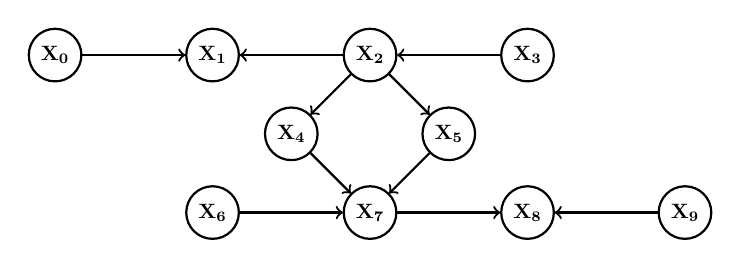
\begin{tikzpicture}[style=thick,scale=1] 
\newcommand{\nsize}{.75}
\begin{scope}[shape=circle,minimum size=0.1cm] 
\tikzstyle{every node}=[draw,fill] 
\node[fill=none,scale=\nsize] (X_0) at (-2,2) {$\mathbf{X_0}$};
\node[fill=none,scale=\nsize] (X_1) at (0,2) {$\mathbf{X_1}$};
\node[fill=none,scale=\nsize] (X_2) at (2,2) {$\mathbf{X_2}$};
\node[fill=none,scale=\nsize] (X_3) at (4,2) {$\mathbf{X_3}$};
\node[fill=none,scale=\nsize] (X_4) at (1,1) {$\mathbf{X_4}$};
\node[fill=none,scale=\nsize] (X_5) at (3,1) {$\mathbf{X_5}$};
\node[fill=none,scale=\nsize] (X_6) at (0,0) {$\mathbf{X_6}$};
\node[fill=none,scale=\nsize] (X_7) at (2,0) {$\mathbf{X_7}$};
\node[fill=none,scale=\nsize] (X_8) at (4,0) {$\mathbf{X_8}$};
\node[fill=none,scale=\nsize] (X_9) at (6,0) {$\mathbf{X_9}$};
\draw [->] (X_0) -- (X_1);
\draw [->] (X_2) -- (X_1);
\draw [->] (X_3) -- (X_2);
\draw [->] (X_2) -- (X_4);
\draw [->] (X_2) -- (X_5);
\draw [->] (X_4) -- (X_7);
\draw [->] (X_5) -- (X_7);
\draw [->] (X_6) -- (X_7);
\draw [->] (X_7) -- (X_8);
\draw [->] (X_9) -- (X_8);
\end{scope} 
\end{tikzpicture}
        \caption{A directed graph}
            \label{fig:bn}
        \end{center}
\end{figure}
\begin{enumerate}[label=(\alph*)]
\item ${\bf A} = \{ X_3 \}$, ${\bf B} = \{ X_4 \}$, ${\bf C} = \{X_1,X_2\}$

\begin{answertext}{2cm}{}
\end{answertext}
\item ${\bf A} = \{ X_5 \}$, ${\bf B} = \{X_4\}$, ${\bf C} = \{X_2,X_7\}$

\begin{answertext}{2cm}{}
\end{answertext}
\item ${\bf A} = \{X_4\}$, ${\bf B} = \{X_6\}$, ${\bf C} = \{X_8\}$

\begin{answertext}{2cm}{}
\end{answertext}
\item ${\bf A} = \{X_5\}$, ${\bf B} = \{X_4\}$, ${\bf C} = \{X_2\}$

\begin{answertext}{2cm}{}
\end{answertext}
\item ${\bf A} = \{X_6, X_9\}$, ${\bf B} = \{X_8\}$, ${\bf C} = \{X_3,X_1\}$

\begin{answertext}{2cm}{}
\end{answertext}
\end{enumerate}


\item Now consider a Markov Random Field as given in Figure~\ref{fig:mrf}, where each edge is undirected. Are the sets ${\bf A}$ and ${\bf B}$ d-separated given set ${\bf C}$ for each of the following definitions of ${\bf A}$, ${\bf B}$ and ${\bf C}$? Justify each answer.

\begin{figure}[h]
    \begin{center}
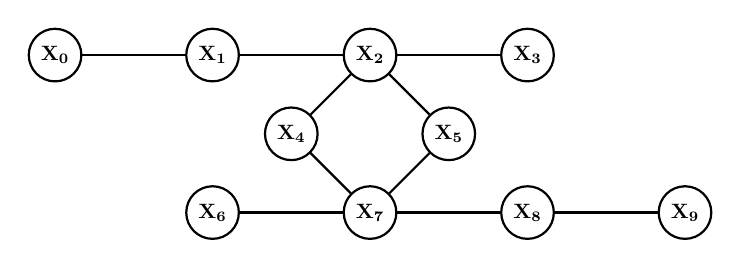
\begin{tikzpicture}[style=thick,scale=1] 
\newcommand{\nsize}{.75}
\begin{scope}[shape=circle,minimum size=0.1cm] 
\tikzstyle{every node}=[draw,fill] 
\node[fill=none,scale=\nsize] (X_0) at (-2,2) {$\mathbf{X_0}$};
\node[fill=none,scale=\nsize] (X_1) at (0,2) {$\mathbf{X_1}$};
\node[fill=none,scale=\nsize] (X_2) at (2,2) {$\mathbf{X_2}$};
\node[fill=none,scale=\nsize] (X_3) at (4,2) {$\mathbf{X_3}$};
\node[fill=none,scale=\nsize] (X_4) at (1,1) {$\mathbf{X_4}$};
\node[fill=none,scale=\nsize] (X_5) at (3,1) {$\mathbf{X_5}$};
\node[fill=none,scale=\nsize] (X_6) at (0,0) {$\mathbf{X_6}$};
\node[fill=none,scale=\nsize] (X_7) at (2,0) {$\mathbf{X_7}$};
\node[fill=none,scale=\nsize] (X_8) at (4,0) {$\mathbf{X_8}$};
\node[fill=none,scale=\nsize] (X_9) at (6,0) {$\mathbf{X_9}$};
\draw [-] (X_0) -- (X_1);
\draw [-] (X_2) -- (X_1);
\draw [-] (X_3) -- (X_2);
\draw [-] (X_2) -- (X_4);
\draw [-] (X_2) -- (X_5);
\draw [-] (X_4) -- (X_7);
\draw [-] (X_5) -- (X_7);
\draw [-] (X_6) -- (X_7);
\draw [-] (X_7) -- (X_8);
\draw [-] (X_9) -- (X_8);
\end{scope} 
\end{tikzpicture}
        \caption{An undirected graph}
            \label{fig:mrf}
        \end{center}
\end{figure}
\begin{enumerate}[label=(\alph*)]
\item ${\bf A} = \{ X_3 \}$, ${\bf B} = \{ X_4 \}$, ${\bf C} = \{X_1,X_2\}$

\begin{answertext}{2cm}{}
\end{answertext}
\item ${\bf A} = \{ X_5 \}$, ${\bf B} = \{X_4\}$, ${\bf C} = \{X_2,X_7\}$

\begin{answertext}{2cm}{}
\end{answertext}
\item ${\bf A} = \{X_4\}$, ${\bf B} = \{X_6\}$, ${\bf C} = \{X_8\}$

\begin{answertext}{2cm}{}
\end{answertext}
\item ${\bf A} = \{X_5\}$, ${\bf B} = \{X_4\}$, ${\bf C} = \{X_2\}$

\begin{answertext}{2cm}{}
\end{answertext}
\item ${\bf A} = \{X_6, X_9\}$, ${\bf B} = \{X_8\}$, ${\bf C} = \{X_3,X_1\}$

\begin{answertext}{2cm}{}
\end{answertext}
\end{enumerate}
\end{enumerate}

}

\end{document}
